% !TEX encoding = UTF-8 Unicode

\documentclass[a4paper]{article}


\usepackage{color}
\usepackage{url}
\usepackage{amsthm}
\usepackage[T2A]{fontenc} % enable Cyrillic fonts
\usepackage[utf8]{inputenc} % make weird characters work
\usepackage{graphicx}
\usepackage{subcaption}
\usepackage{amsmath}
\usepackage{verbatim}
\usepackage{array}
\usepackage[table]{xcolor}
\usepackage{float}

\graphicspath{ {./images/} }

\usepackage[english,serbian]{babel}

\usepackage[unicode]{hyperref}


%================= start config for code printing
\usepackage{listings}
\usepackage{color}

\definecolor{dkgreen}{rgb}{0,0.6,0}
\definecolor{gray}{rgb}{0.5,0.5,0.5}
\definecolor{mauve}{rgb}{0.58,0,0.82}

\lstset{frame=tb,
  language=Java,
  aboveskip=3mm,
  belowskip=3mm,
  showstringspaces=false,
  columns=flexible,
  basicstyle={\small\ttfamily},
  numbers=none,
  numberstyle=\tiny\color{gray},
  keywordstyle=\color{blue},
  commentstyle=\color{dkgreen},
  stringstyle=\color{mauve},
  breaklines=true,
  breakatwhitespace=true,
  tabsize=4
}

%============ end code

\hypersetup{colorlinks,citecolor=green,filecolor=green,linkcolor=blue,urlcolor=blue}

\newtheorem*{tvrdjenje}{Tvrđenje}
\newtheorem*{hipoteza}{Hipoteza}
\theoremstyle{definition}
\newtheorem{primer}{Primer}[section]



\begin{document}

\title{YouTube Trending\\ \small{Seminarski rad u okviru kursa\\Istraživanje podataka\\ Matematički fakultet}}

\author{Nikola Dimitrijević \footnote{mi14079@alas.matf.bg.ac.rs}\\
        Luka Živanović \footnote{mi14164@alas.matf.bg.ac.rs}\\
 }
%\date{9.~april 2015.}
\vspace*{-3cm}
    {\let\newpage\relax\maketitle}

\tableofcontents

\newpage



% ==============================================================================
\section{Uvod}
\label{sec:uvod}
% ==============================================================================
Skup podataka ``Trending YouTube Video Statistics'' sadrži informacije o YouTube video klipovima koji su se pojavili na trending listi.
Klipovi koji se nalaze na trendingu su u tom trenutku aktuelni, popularni ili relevantni. Neće svaki klip sa mnogo pregleda biti na trendingu,
 pritom se trending liste razlikuju za svaku državu. Podaci su nastali višemesečnim prikupljanjem klipova sa trending liste korišćenjem YouTube API.
Skup podataka se može naći na adresi \url{https://www.kaggle.com/datasnaek/youtube-new}.
Za obradu tokom ovog projekta su korišćeni KNIME platforma i Java programski jezik.

Prvo će biti dat opis podataka, potom pregled KNIME projekta i kako je rađeno pretprocesiranje. Nakon toga će biti prikazano korišćenje algoritama i njihovi rezultati, a na kraju
vizuelizacije podataka.
% ==============================================================================
\section{Analiza i pretprocesiranje podataka}


\label{sec:analiza}
% ==============================================================================

\subsection{Opis skupa podataka}
Podaci se nalaze u više tabela: US, GB, DE,
CA i FR (SAD, Velika Britanija, Nemačka, Kanada i Francuska redom).
Svaki klip se može naći više puta na trendingu.
Primera radi, US tabela sadrži 38549 redova, među kojima je zapravo  6201 različitih klipova.


\begin{table}[H]
\centering
\begin{tabular}{ |c|c| }
 \hline
 video\_id & jedinstveni identifikator svakog video klipa  \\
\hline
 trending\_date & datum kad je klip bio na trendingu (yy.dd.mm)  \\
\hline
 title & naziv klipa  \\
\hline
 channel\_title & naziv kanala koji je postavio klip  \\
\hline
 category\_id & jedinstveni identifikator tematske kategorije klipa  \\
\hline
publish\_time & vreme postavljanja klipa (yyyy-mm-ddThh:mm:ss.000Z)\\
\hline
tags & ključne reči, u formatu tag1|tag2|... |tagn  \\
\hline
views & broj pregleda  \\
\hline
likes & broj ljudi koji su izabrali da im se sviđa klip\\
\hline
dislikes & broj ljudi koji su izabrali da im se ne sviđa klip   \\
\hline
comment\_count & broj komentara \\
\hline
thumbnail\_link & link ka sličici koja predstavlja video klip  \\
\hline
comments\_disabled & da li su komentari isključeni  \\
\hline
ratings\_disabled & da li je ocenjivanje isključeno \\
\hline
video\_error\_or\_removed & da li video ima grešku ili je uklonjen  \\
\hline
description & opis video klipa  \\
 \hline
\end{tabular}
\caption{Opis datoteke USvideos.csv. Nazivi kolona su dati levo, a njihovi opisi desno.}
\label{table:1}
\end{table}

Ovaj skup podataka takođe sadrži i JSON datoteke za svaku od navedenih država.
Razlog za to je što se skup tematskih kategorija klipova razlikovao među državama, pa se u JSON datotekama nalaze imena koja odgovaraju određenim identifikatorima kategorija.

\subsection{Pretprocesiranje} \label{pretprocesiranje}

\begin{figure}[H]
\begin{center}
    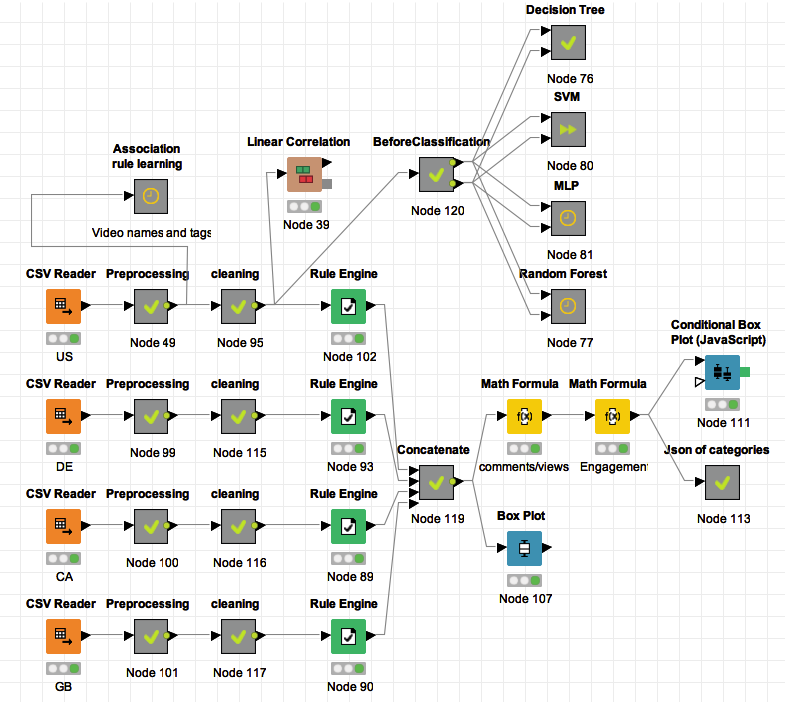
\includegraphics[width=1\textwidth]{Global.png}
    \caption{Globalni pogled na KNIME projekat}
    \label{fig:global}
\end{center}
\end{figure}

U donjem levom delu se učitavaju podaci iz .csv datoteka, pretprocesiraju, prečišćavaju, dodaje se redovima oznaka na koju državu se odnose.
Nakon toga se svi spajaju u jednu ogrmonu tabelu.

Preprocessing meta-čvor sadrži obrade koje su potrebne za sav dalji tok analize.


\begin{figure}[H]
\begin{center}
    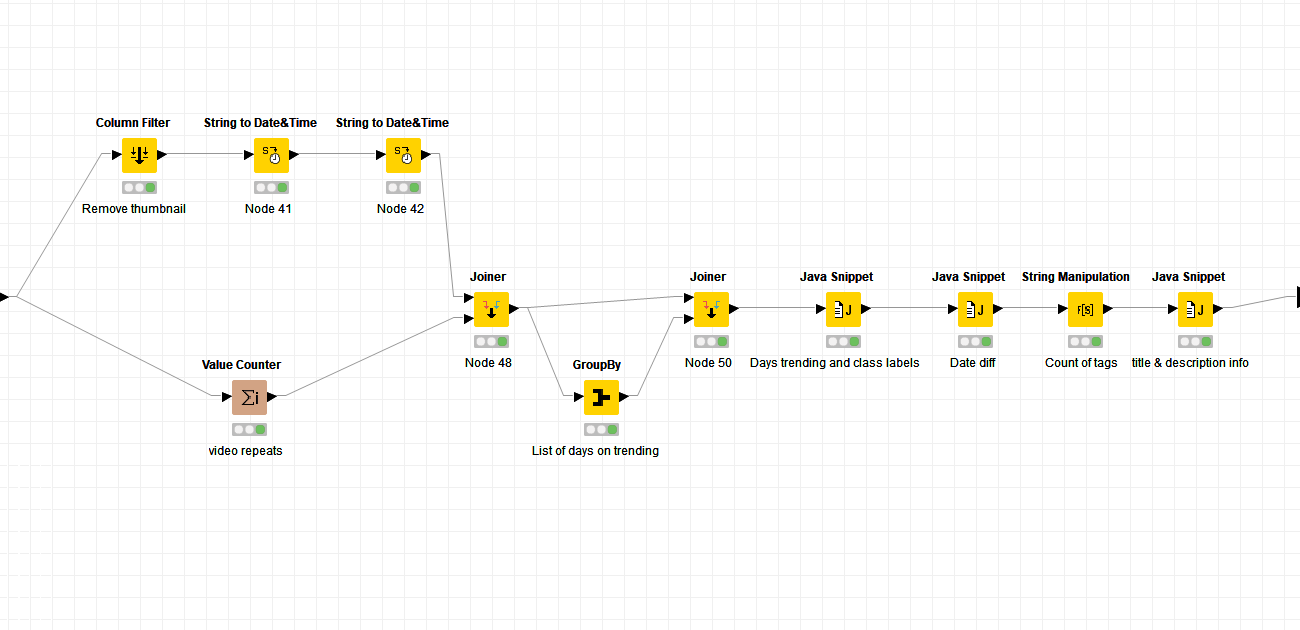
\includegraphics[width=1\textwidth]{preprocessing.png}
    \caption{Pretprocesiranje}
\end{center}
\end{figure}
Prvo se uklanja kolona sa linkom na sliku pošto se to neće koristiti. Potom se konvertuju stringovski zapisi datuma u datumske tipove.
Za svaki video\_id se broji koliko puta se pojavljuje u toj tabeli, pa se potom spajaju kako bi se na sve redove nadovezao taj atribut.
Takođe se izdvaja i lista svih datuma kad je taj klip bio na trendingu.
Za neke operacije nije bilo dovoljno koristiti ugrađene operacije preko običnih KNIME  čvorova, pa se tada koristi ``Java snippet''.

\begin{lstlisting}
// racunanje broja dana koliko je ova instanca bila na trendingu, i da li ce biti jos barem jednom
public void snippet() throws TypeException, ColumnException, Abort {

	// datum trendinga ove instance
	LocalDate l = c_trending_date;
	// lista svih datuma kada je ovaj video_id bio na trendingu
	LocalDate list[] = c_Sortedlisttrending_date;

	int c = 0;
	// brojanje koliko instanci je bilo na trendingu pre ove instance
	for (LocalDate e : c_Sortedlisttrending_date){
		if (l.compareTo(e) >= 0 ){
			c++;
		}
	}
	out_days_trending = c;
	// ako je ova instanca ima najnoviji datum medju svim u listi
	// onda nece biti na trendingu jos jednom
	out_WillTrendAgain = c < list.length ? "true" : "false";

}

\end{lstlisting}


Takođe je pravljen novi atribut koji govori o broju dana između postavljanja klipa na YouTube i dana kada je na trendingu.
Sledeći Java snippet to obrađuje.

\begin{lstlisting}
import java.time.temporal.*;
// system variables
public class JSnippet extends AbstractJSnippet {
// Fields for input columns
/** Input column: "trending_date" */
public LocalDate c_trending_date;
/** Input column: "publish_time" */
public ZonedDateTime c_publish_time;

// Fields for output columns
/** Output column: "days_after_publish" */
public Integer out_days_after_publish;

public void snippet() throws TypeException, ColumnException, Abort {

	long daysBetween = ChronoUnit.DAYS.
		between(c_publish_time.toLocalDate(), c_trending_date);

	out_days_after_publish = (int)daysBetween;
}
\end{lstlisting}

Potom se računa broj tagova, korišćenjem kratkog izraza unutar String Manipulation čvora.

\begin{verbatim}
count($tags$, "|") + compare($tags$, "")
\end{verbatim}

I na kraju se računa više novih atributa korišćenjem sledećeg Java koda.

Cilj je izračunati neke interesantne atribute analizom teksta naziva klipa kao i njegovog opisa.


\begin{lstlisting}
// broj reci u naslovu
out_title_word_count = 0;

// broj reci u naslovu koje pocinju velikim slovom
out_title_capital_percentage = 0.;

// broj reci koje su u potpunosti napisane velikim slovima
out_title_upper_case_percentage = 0.;

// broj reci u opisu klipa
out_description_word_count = 0;

// broj reci u opisu koje pocinju velikim slovom
out_description_capital_percentage = 0.;

// broj reci u opisu koje su u potpunosti napisane velikim slovima
out_description_upper_case_percentage = 0.;

int title_capital_count = 0;
int title_upper_count = 0;
int description_capital_count = 0;
int description_upper_count = 0;

// izdvajaju se grupe karaktera koje su sacinjene 1+ slova
String[] title_words = c_title.split("\\W+");
for (int i=0; i<title_words.length; i++) {
	out_title_word_count++;
	String word = title_words[i];
	int n = word.length();
	boolean isUpper = true;
	boolean isCapital = true;
	for (int j=0; j<n; j++) {
		if (j==0 && word.charAt(j)!=Character.toUpperCase(word.charAt(j))) {
			isUpper = false;
			isCapital = false;
			break;
		} else if (j!=0) {
			if (word.charAt(j)==Character.toUpperCase(word.charAt(j))) {
				isCapital = false;
			}
			else {
				isUpper = false;
			}
		}
	}
	if (isUpper)
		title_upper_count++;
	if (isCapital)
		title_capital_count++;
}

// izdvajaju se grupe karaktera koje su sacinjene 1+ slova
String[] desc_words = c_description.split("\\W+");
for (int i=0; i<desc_words.length; i++) {
	out_description_word_count++;
	String word = desc_words[i];
	int n = word.length();
	boolean isUpper = true;
	boolean isCapital = true;
	for (int j=0; j<n; j++) {
		if (j==0 && word.charAt(j)!=Character.toUpperCase(word.charAt(j))) {
			isUpper = false;
			isCapital = false;
			break;
		} else if (j!=0) {
			if (word.charAt(j)==Character.toUpperCase(word.charAt(j))) {
				isCapital = false;
			}
			else {
				isUpper = false;
			}
		}
	}
	if (isUpper)
		description_upper_count++;
	if (isCapital)
		description_capital_count++;
}

// ako nije bilo nijedne utf-8 reci u naslovu
if (out_title_word_count == 0){
	out_title_capital_percentage = 0.0;
	out_title_upper_case_percentage = 0.0;
} else {
	out_title_capital_percentage = title_capital_count*1.0/out_title_word_count;
	out_title_upper_case_percentage = title_upper_count*1.0/out_title_word_count;

}

// ako nije bilo nijedne utf-8 reci u opisu
if (out_description_word_count == 0){
	out_description_capital_percentage = 0.0;
	out_description_upper_case_percentage = 0.0;
} else {
	out_description_capital_percentage = description_capital_count*1.0/out_description_word_count;
	out_description_upper_case_percentage = description_upper_count*1.0/out_description_word_count;
}


\end{lstlisting}


Meta-čvor za čiščenje sadrži sledeće.

\begin{figure}[H]
\begin{center}
    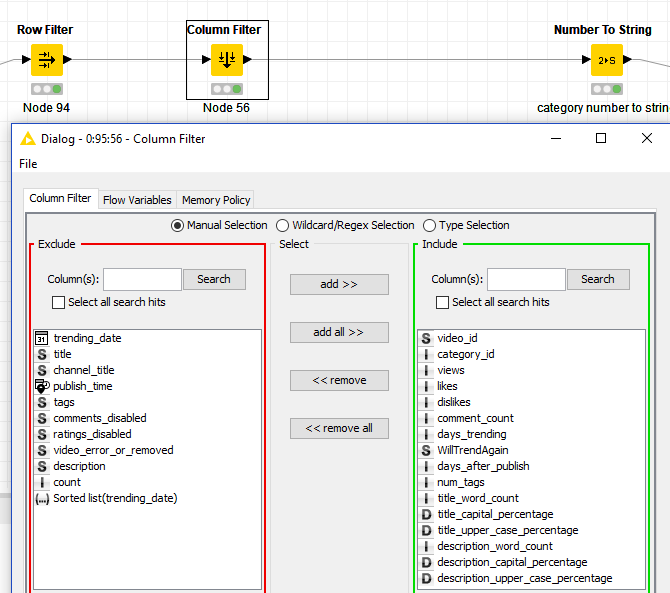
\includegraphics[width=1\textwidth]{cleaning.png}
    \caption{Filtriranje sada nepotrebnih kolona}
\end{center}
\end{figure}

Row filter otklanja 7 neodgovarajućih redova, dok poslednji čvor konvertuje celobrojni zapis identifikatora kategorije u
stringovski, kako bi se posmatrao kao kategorički atribut.

Nakon pretprocesiranja i čišćenja svih csv datoteka potrebno ih je spojiti u jednu veliku tabelu. To se dešava unutar concatenate meta-čvora.

\begin{figure}[H]
\begin{center}
    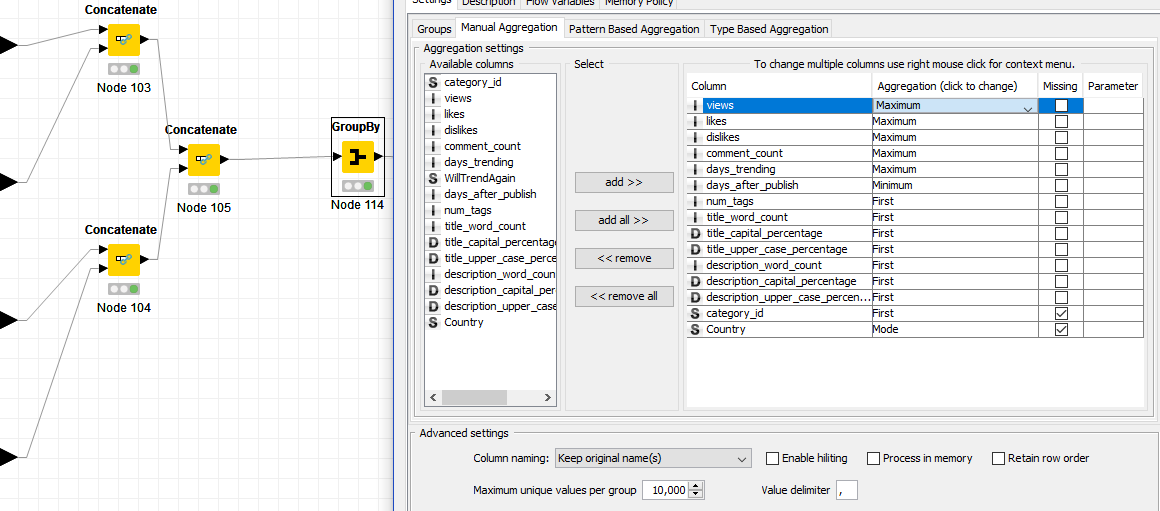
\includegraphics[width=1\textwidth]{concatenation.png}
    \caption{Sadržaj concatenate meta-čvora i detalji grupisanja}
    \label{fig:concat}
\end{center}
\end{figure}

Na kraju su video klipovi grupisani tako da se jedan video\_id nalazi samo u jednom redu, detalji grupisanja su prikazani na slici \ref{fig:concat}.

Da bi se dobili odgovarajuci nazivi tematskih kategorija video klipova potrebno je spojiti csv redove sa redovima iz JSON datoteka.
Nakon ucitavanja JSON datoteke, potrebno je idvojiti sve elemente niza korišćenjem JSON Path selektora.
Tada je na raspolaganju samo jedan red koji sadrži sve JSON objekte koji čine pomenuti niz.
Pomoću ungroup čvora dobija se više redova gde svaki predstavlja jedan element početnog niza.
Ponovnim korišćenjem JSON path selektora dobija se tabela koja u svakom redu umesto jednog JSON objekta
sada ima dva atributa. Jedan je identifikator kategorije, a drugi je njen naziv na engleskom.
\begin{figure}[H]
\begin{center}
    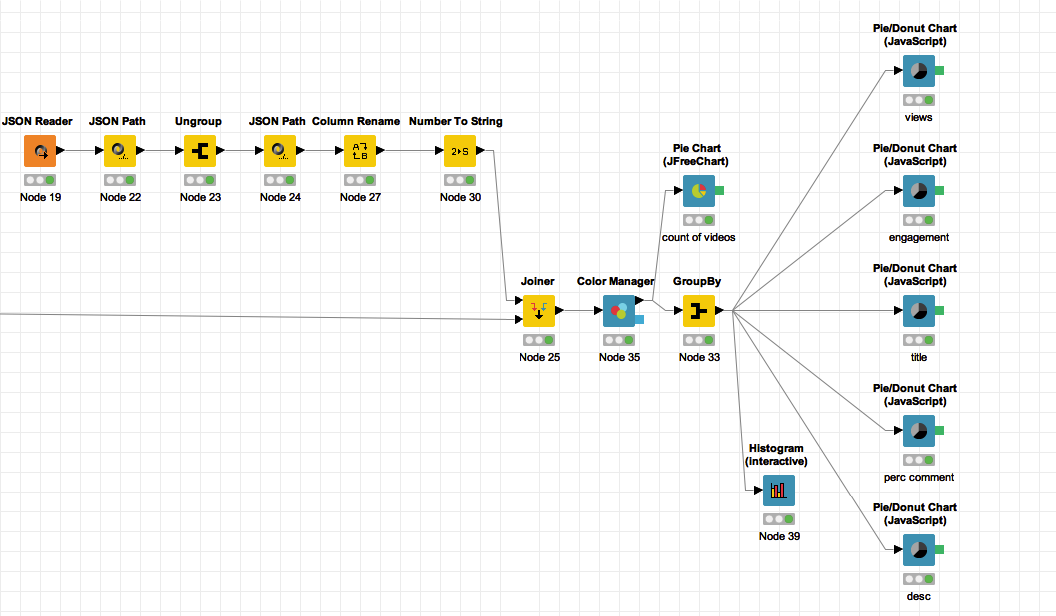
\includegraphics[width=1\textwidth]{json_of_categories.png}
    \caption{Pretprocesiranje JSON datoteka}
    \label{fig:json}
\end{center}
\end{figure}


% ==============================================================================
\section{Klasifikacija}
\label{sec:klasifikacija}
% ==============================================================================
Nakon pretprocesiranja i čišćenja podataka, pre same klasifikacije izbacuje se atribut \textit{video\_id}, normalizuju se podaci koji se dele na skup za obučavanje i skup za testiranje.

\begin{figure}[H]
\begin{center}
    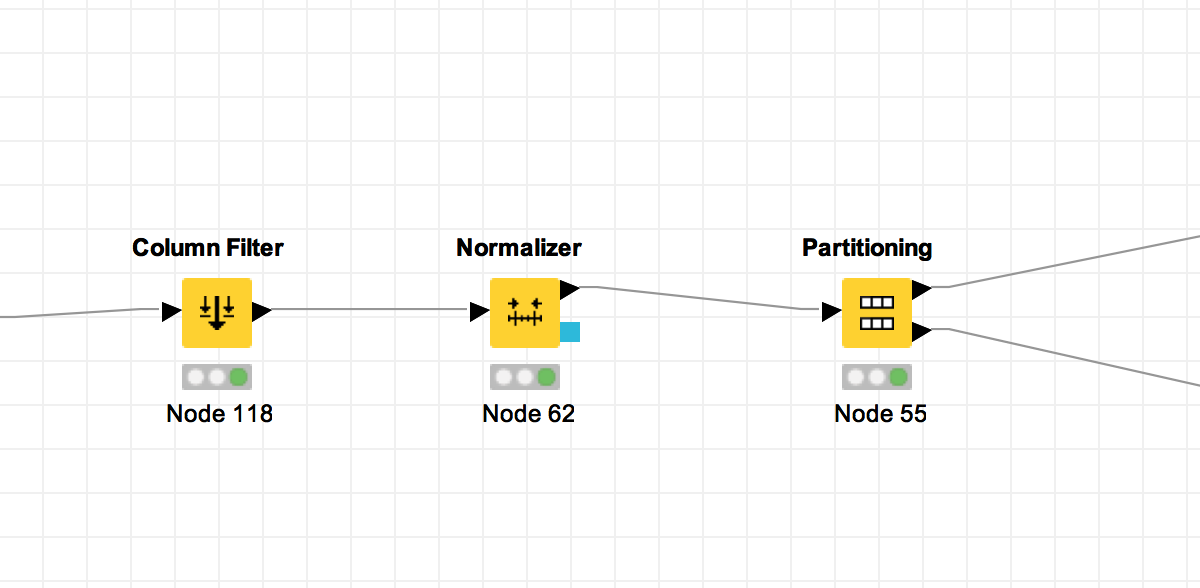
\includegraphics[width=1\textwidth]{before_classification.png}
    \caption{Priprema podataka za klasifikaciju}
\end{center}
\end{figure}

Koristeći tako modifikovane podatke, četiri algoritma će pokušati da predvide da li će video ponovo biti na trendingu. Svi meta parametri su podešeni kako bi se dobili što bolji rezultati, a konačni rezultati za svaki metod klasifikacije su:

\begingroup

\renewcommand\arraystretch{1.3}

\noindent\begin{tabular}{
  | >{\ttfamily}p{2.2cm}
  | >{\sffamily}p{2.2cm}
  | >{\sffamily}p{5.85cm} |
}
\hline
\rowcolor{gray!20}\multicolumn{1}{|l|}{\bfseries\sffamily Algoritam}
  & \multicolumn{1}{l|}{\bfseries\sffamily Tačnost}
  & \multicolumn{1}{l|}{\bfseries\sffamily Matrica konfuzije} \\
\hline
& & \\[-2ex]
Stablo odlučivanja \newline str:\pageref{fig:stabloOdlucivanja} & 83.648\%  &
  \begin{tabular}[t]{
    | >{\ttfamily\raggedright}p{1.5cm}
    | >{\sffamily\raggedright}p{1.5cm}
    | >{\sffamily}p{1.5cm} |
  }
  \firsthline
    & \multicolumn{1}{l|}{\cellcolor{gray!20} tačno}
    & \multicolumn{1}{l|}{\cellcolor{gray!20} netačno}  \\
  \hline
  \cellcolor{gray!20} tačno  & 9547 & 150 \\
  \hline
  \cellcolor{gray!20} netačno  & 1740 & 121 \\
  \hline
  \end{tabular} \\[10ex]

\hline
\rowcolor{gray!20}\multicolumn{1}{|l|}{\bfseries\sffamily Algoritam}
  & \multicolumn{1}{l|}{\bfseries\sffamily Tačnost}
  & \multicolumn{1}{l|}{\bfseries\sffamily Matrica konfuzije} \\
\hline
& & \\[-2ex]
SVM \newline str:\pageref{fig:SVM}  & 83.899\% &
  \begin{tabular}[t]{
    | >{\ttfamily\raggedright}p{1.5cm}
    | >{\sffamily\raggedright}p{1.5cm}
    | >{\sffamily}p{1.5cm} |
  }
  \firsthline
    & \multicolumn{1}{l|}{\cellcolor{gray!20} tačno}
    & \multicolumn{1}{l|}{\cellcolor{gray!20} netačno}  \\
  \hline
  \cellcolor{gray!20} tačno  & 9697 & 0 \\
  \hline
  \cellcolor{gray!20} netačno  & 1861 & 0 \\
  \hline
  \end{tabular} \\[10ex]

\hline
\rowcolor{gray!20}\multicolumn{1}{|l|}{\bfseries\sffamily Algoritam}
  & \multicolumn{1}{l|}{\bfseries\sffamily Tačnost}
  & \multicolumn{1}{l|}{\bfseries\sffamily Matrica konfuzije} \\
\hline
& & \\[-2ex]
MLP \newline str:\pageref{fig:MLP}  & 83.708\% &
  \begin{tabular}[t]{
    | >{\ttfamily\raggedright}p{1.5cm}
    | >{\sffamily\raggedright}p{1.5cm}
    | >{\sffamily}p{1.5cm} |
  }
  \firsthline
    & \multicolumn{1}{l|}{\cellcolor{gray!20} tačno}
    & \multicolumn{1}{l|}{\cellcolor{gray!20} netačno}  \\
  \hline
  \cellcolor{gray!20} tačno  & 9659 & 37 \\
  \hline
  \cellcolor{gray!20} netačno  & 1844 & 16 \\
  \hline
  \end{tabular} \\[10ex]

\hline
\rowcolor{gray!20}\multicolumn{1}{|l|}{\bfseries\sffamily Algoritam}
  & \multicolumn{1}{l|}{\bfseries\sffamily Tačnost}
  & \multicolumn{1}{l|}{\bfseries\sffamily Matrica konfuzije} \\
\hline
& & \\[-2ex]
Random Forrest \newline str:\pageref{fig:randomForrest}  & 83.656\% &
  \begin{tabular}[t]{
    | >{\ttfamily\raggedright}p{1.5cm}
    | >{\sffamily\raggedright}p{1.5cm}
    | >{\sffamily}p{1.5cm} |
  }
  \firsthline
    & \multicolumn{1}{l|}{\cellcolor{gray!20} tačno}
    & \multicolumn{1}{l|}{\cellcolor{gray!20} netačno}  \\
  \hline
  \cellcolor{gray!20} tačno  & 9633 & 64 \\
  \hline
  \cellcolor{gray!20} netačno  & 1825 &  36 \\
  \hline
  \end{tabular} \\[10ex]

\hline
\end{tabular}
\\ \\
\endgroup


Svaki od metačvorova ima svoj Learner čvor, koji koristeći podatke sa trening skupa kreira model, koji se potom primenjuje na trening i test skupove, kako bi se njihovi rezultati uporedili.
\\ \\
Primećuje se da su svi parametri konfigurisani tako da nema mnogo preprilagođavanja ni potprilagođavanja, ali tačnost na trening skupovima ne prelazi 85\%. Situacija je takva pošto, iako dati skupovi imaju veliki broj redova i kolona, određeni parametri koji određuju da li će video biti u trendingu ne postoje, poput lokacije svakog pregleda. Čak i sa tim informacijama, moguće je da tačnost ne bi postigla dovoljno visoki stepen, zato što nije poznato kako funkcioniše Youtube-ov algoritam za postavljanje videa na trending.
\\ \\
Takođe, treba primetiti da se algoritam stablo odlučivanja i Random Forrest izvršavaju za manje od jednog minuta, MLP sa 3 skrivena sloja i 500 iteracija za 3 minuta, dok je SVM algoritmu, čiji je ulaz transformisan PCA procedurom na 4 dimenzije sa očuvanih 95\% podataka, potrebno više od 90 minuta na istom računaru i ima najlošije rezultate. Ovakav rezultat je posledica kompleksnosti SVM algoritma i nemogućnosti za finim podešavanjem parametara zbog dužine izvršavanja.

% KLASIFIKACIJA

\begin{figure}[H]
\begin{center}
    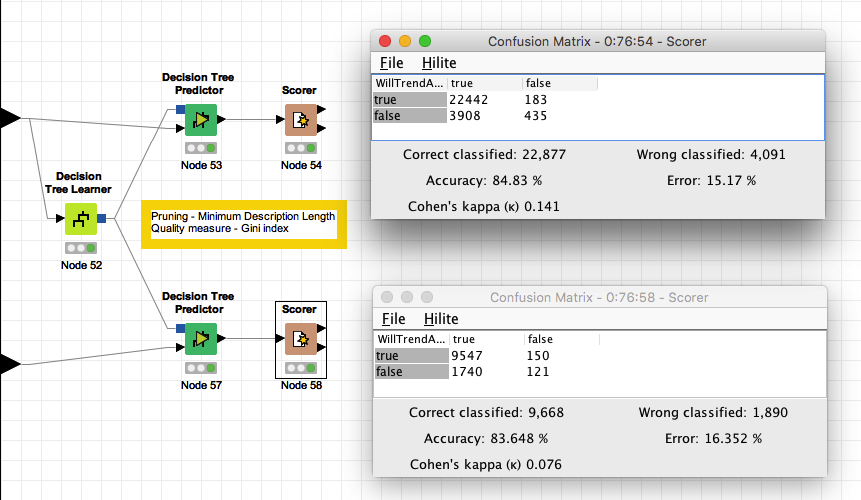
\includegraphics[width=1\textwidth]{decision_tree.png}
    \caption{Stablo odlučivanja}
\end{center}
\label{fig:stabloOdlucivanja}
\end{figure}

\begin{figure}[H]
\begin{center}
    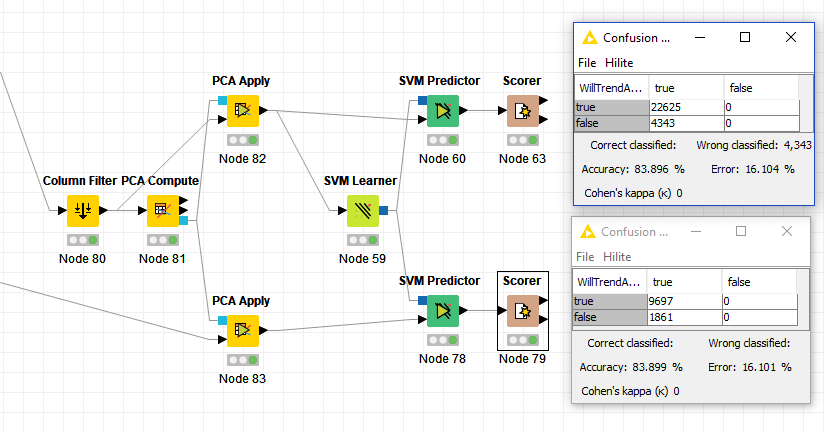
\includegraphics[width=1\textwidth]{SVM.png}
    \caption{SVM}
\end{center}
\label{fig:SVM}
\end{figure}

\begin{figure}[H]
\begin{center}
    \includegraphics[width=1\textwidth]{MLP.png}
    \caption{MLP}
\end{center}
\label{fig:MLP}
\end{figure}

\begin{figure}[H]
\begin{center}
    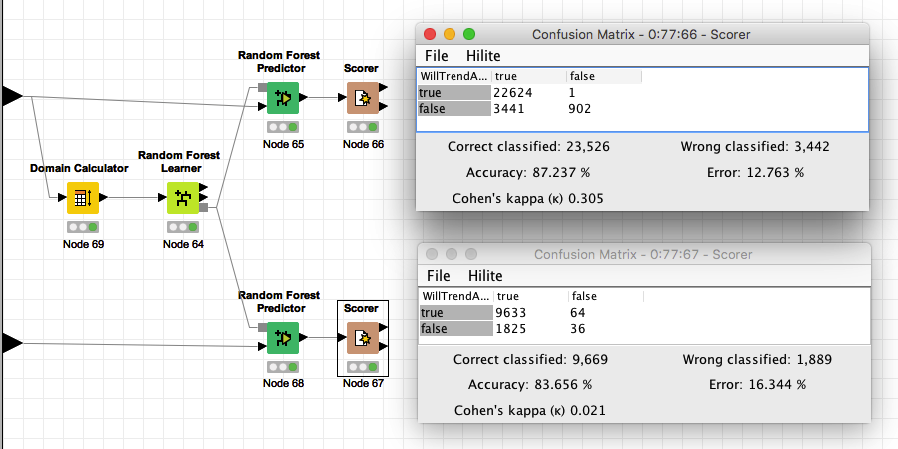
\includegraphics[width=1\textwidth]{Random_Forrest.png}
    \caption{Random Forrest}
\end{center}
\label{fig:randomForrest}
\end{figure}


% ==============================================================================
\section{Pravila pridruživanja}
\label{sec:pravila}
% ==============================================================================

Transformacijom niski tagova i naslova u nizove i primenom algoritma za generisanje pravila pridruživanja dobili smo rezultate: \ref{fig:asoc1}, \ref{fig:asoc2}.
\\
Kako ne pokušavamo da uočimo pravila engleskog jezika, izbacili smo iz pretrage reči a, is, the, an, to, of, in, and, with, on.
\begin{lstlisting}
String skip[] = {"a", "is", "the", "an", "", " ", "to", "of", "in", "and", "with", "on"};
\end{lstlisting}
Takođe, reči su transformisane tako da sadrže samo mala slova i da ne sadrže specijalne karaktere osim ', kako bi algoritam mogao da generalizuje što bolje pravila, umesto da da kreira nova zbog kreativnih naslova koji se neretko javljaju.

% ASOC

\begin{figure}[H]
\begin{center}
    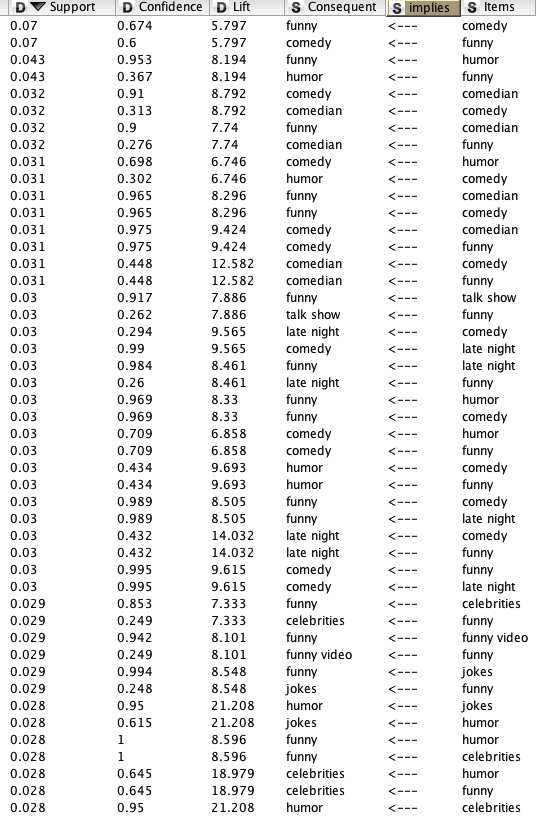
\includegraphics[width=1\textwidth]{association.png}
    \caption{Asocijacija - Naslovi}
    \label{fig:asoc1}
\end{center}
\end{figure}

\begin{figure}[H]
\begin{center}
    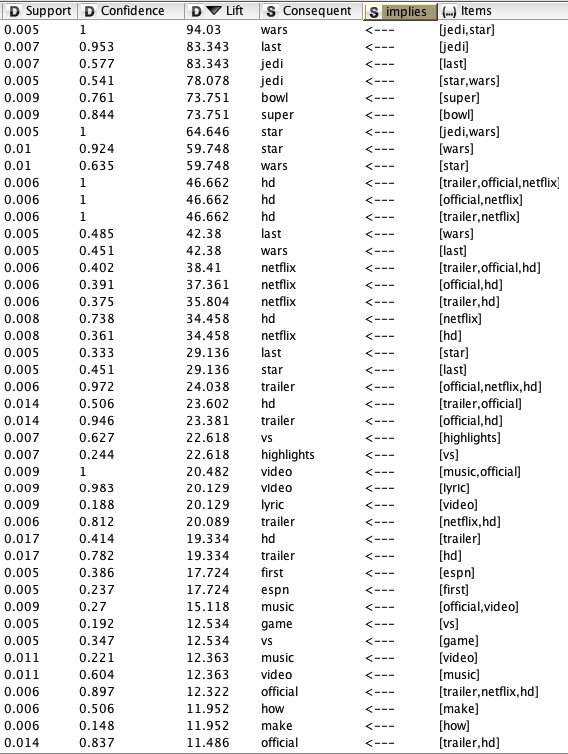
\includegraphics[width=1\textwidth]{association2.png}
    \caption{Asocijacija - Tagovi}
     \label{fig:asoc2}
\end{center}
\end{figure}

% ==============================================================================
\section{Klasterovanje}
\label{sec:dod}
% ==============================================================================

Klasterovanje je rađeno korišteći SPSS Modeler pošto ima robustnan sistem za taj zadatak.

% ==============================================================================
\section{Vizuelizacije podataka}
\label{sec:dod}
% ==============================================================================

U nastavku će se koristiti termin koji nije ranije definisan - \textbf{angažovanost}:
\newline

$$\text{angažovanost} = \frac{\text{broj lajkova} + \text{broj dislajkova} + \text{broj komentara}}{\text{broj pregleda}}$$

Na slici \ref{fig:global} se vide dva Math Formula čvora, koji računaju dva nova atributa koje je zanimljivo analizirati.
Angažovanost označava koliko su gledaoci određenog klipa aktivni na njemu. Na englsekom se naziva engagement i
bitna je metrika za ljude koji žele da njihovi kanali budu što popularniji.


\subsection{Vizuelizacije numeričkih podataka}

Na slikama od \ref{fig:boxDesc} do \ref{fig:boxEngagement} možemo videti vizuelizaciju nekih osobina video klipova poput broja reči u opisu i naslovu, broja tagova, dana koliko je video bio u trendingu i angažovanost po državama. Na svakoj slici se pojavljuje veliki broj elemenata van granice. Što se tiče broja reči i tagova, jasno je da postoji veliki broj takvih elemenata, zato što Youtube-ov algoritam mora da bude nepoznat ljudima, odnosno, ukoliko bi favorizovao neku predefinisanu granicu, kreatori klipova bi se držali toga, što Youtube-u nije cilj.
\\
Što se tiče dana u trendingu i angažovanosti, i ti podaci su očekivani zbog socijalnog aspekta. Ponekad se pojavi klip koji izazove burne reakcije i on bude duže na trendingu, ali obično nije takav slulčaj. Što se angažovanosti tiče, takođe se javljaju klipovi koji izazivaju veliki broj komentara i obično dislajkova, koji odstupaju od granice.

\subsection{Vizuelizacije po kategorijama}

U sekciji pretrprocesiranje (\ref{pretprocesiranje}) je opisan proces dodavanja kategorija u skup video klipova.

Na slikama \ref{fig:brojKlipova} i \ref{fig:brojPregleda} se može primetiti da većinu ne predstavlja ista kategorija. Takva informacija je i očekivana, zato što se pesme ne objavljuju često koliko zabavni klipovi, ali se preslušavaju daleko češće.

% VIZUELIZACIJA NUM

\begin{figure}[H]
\begin{center}
    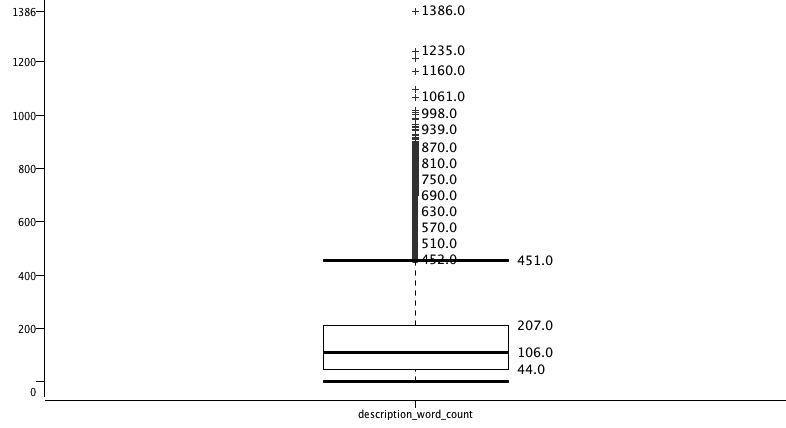
\includegraphics[width=1\textwidth]{box_desc_word_count.png}
    \caption{Broj reči u opisu}
    \label{fig:boxDesc}
\end{center}
\end{figure}

\begin{figure}[H]
\begin{center}
    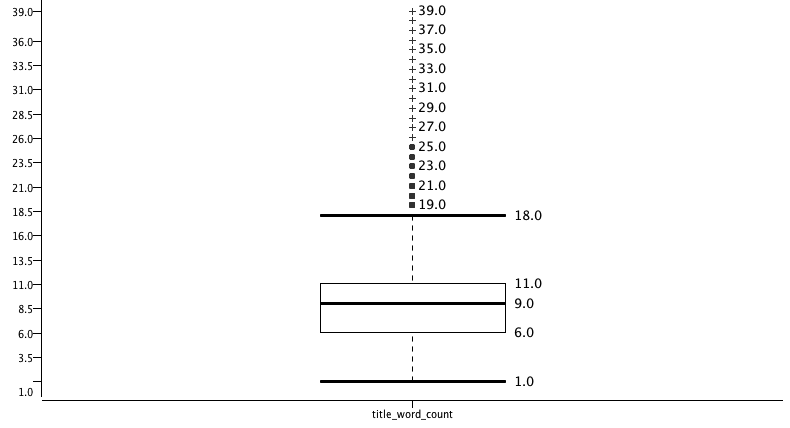
\includegraphics[width=1\textwidth]{box_title_word_count.png}
    \caption{Broj reči u naslovu}
\end{center}
\end{figure}

\begin{figure}[H]
\begin{center}
    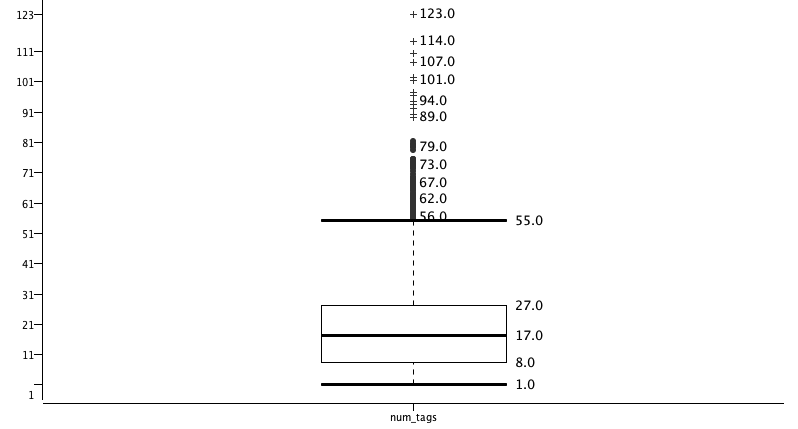
\includegraphics[width=1\textwidth]{box_num-tag.png}
    \caption{Broj tagova}
\end{center}
\end{figure}

\begin{figure}[H]
\begin{center}
    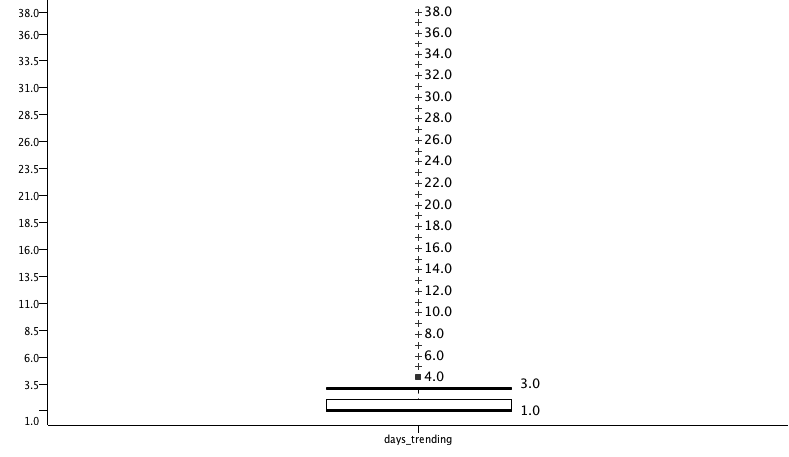
\includegraphics[width=1\textwidth]{box_trending.png}
    \caption{Dani u trendingu}
\end{center}
\end{figure}

\begin{figure}[H]
\begin{center}
    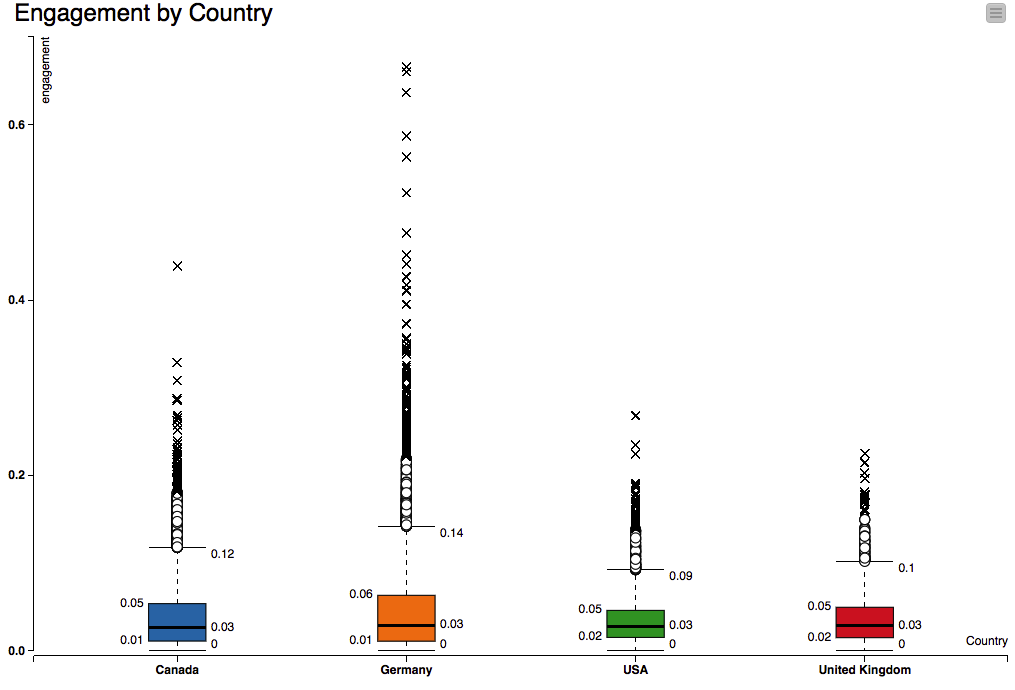
\includegraphics[width=1\textwidth]{engagement_box_plot.png}
    \caption{Angažovanost po državi}
        \label{fig:boxEngagement}
\end{center}
\end{figure}






%VIZUELIZACIJA KAT

\begin{figure}[H]
\begin{center}
    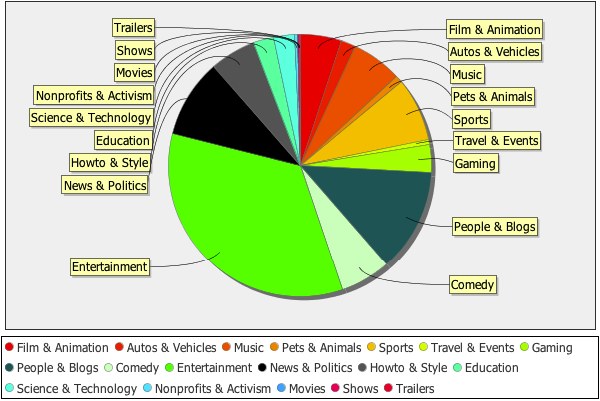
\includegraphics[width=1\textwidth]{categories_clips.png}
    \caption{Broj klipova po kategorijama}
    \label{fig:brojKlipova}
\end{center}
\end{figure}

\begin{figure}[H]
\begin{center}
    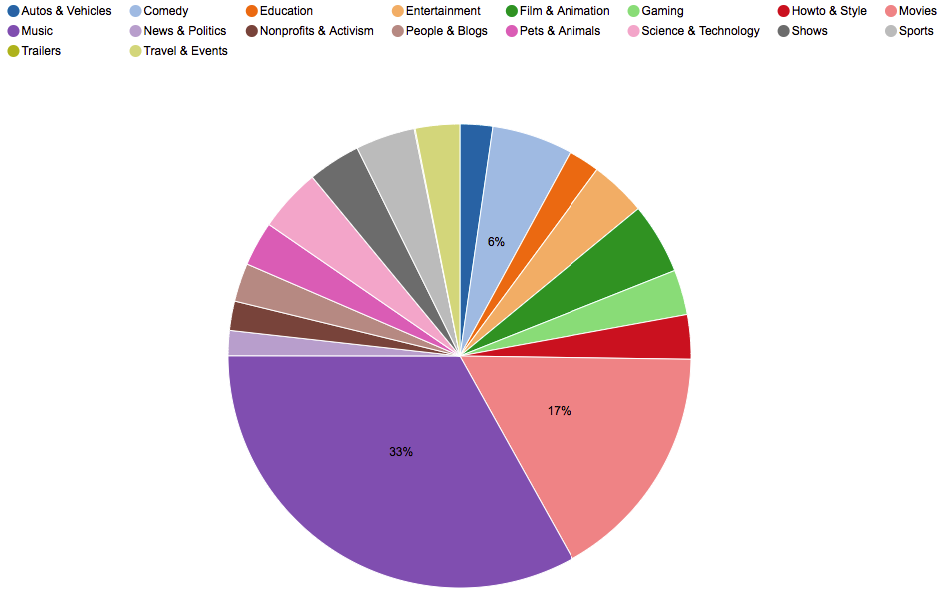
\includegraphics[width=1\textwidth]{categories_views.png}
    \caption{Broj pregleda po kategorijama}
    \label{fig:brojPregleda}
\end{center}
\end{figure}

\begin{figure}[H]
\begin{center}
    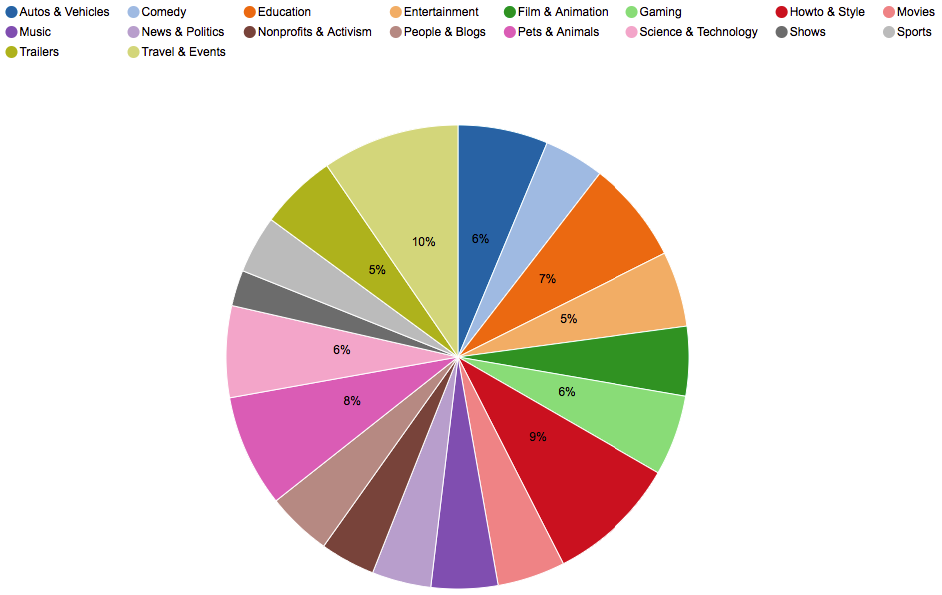
\includegraphics[width=1\textwidth]{categories_desc.png}
    \caption{Broj reči u opisu po kategorijama}
\end{center}
\end{figure}

\begin{figure}[H]
\begin{center}
    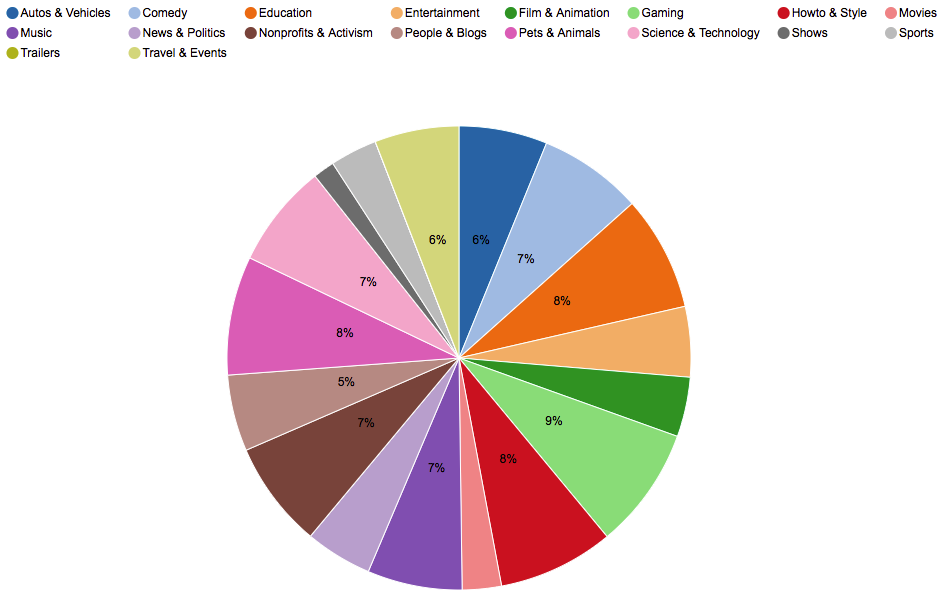
\includegraphics[width=1\textwidth]{categories_engagement.png}
    \caption{Angažovanost po kategorijama}
\end{center}
\end{figure}

\begin{figure}[H]
\begin{center}
    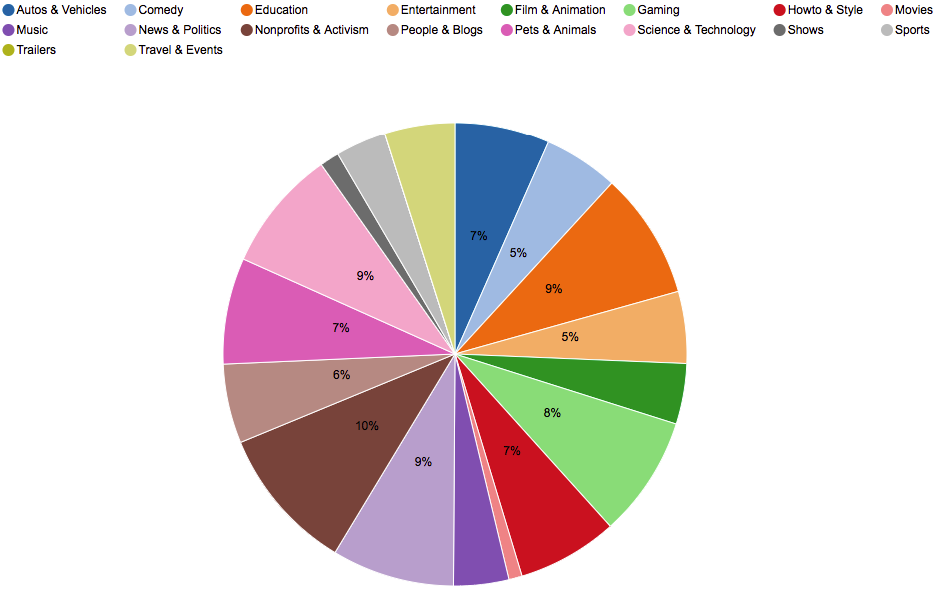
\includegraphics[width=1\textwidth]{categories_perc-title.png}
    \caption{Odnos broja komentara i pregleda po kategoriji }
\end{center}
\end{figure}

\begin{figure}[H]
\begin{center}
    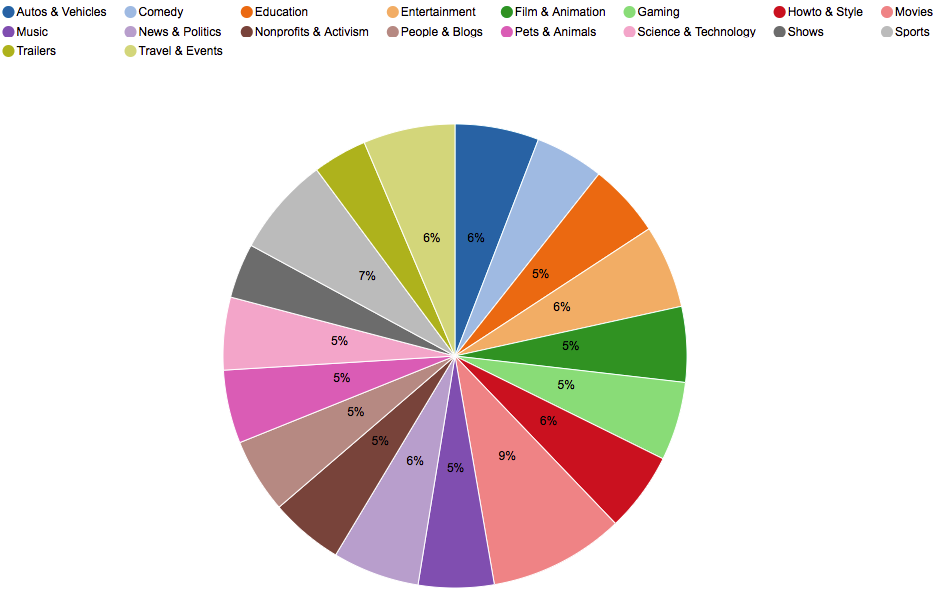
\includegraphics[width=1\textwidth]{categories_title.png}
    \caption{Broj reči u naslovu po kategoriji}
\end{center}
\end{figure}

\end{document}
